\documentclass[a4paper,11pt ]{book}
\usepackage[T1]{fontenc}
\usepackage[utf8]{inputenc}
\usepackage{lmodern}
\usepackage{amsmath}
\usepackage{amsfonts}
\usepackage{amssymb}
\usepackage{amsthm}
\usepackage{graphicx}
\usepackage{color}
\usepackage{xcolor}
\usepackage{url}
\usepackage{theorem}
\usepackage{textcomp}
\usepackage{glossaries}
\usepackage{parskip}
\usepackage{xlop}
\usepackage{multicol}
\graphicspath{ {./Images/} }
\usepackage{tikz}
\usetikzlibrary{decorations.pathreplacing,calligraphy,decorations.pathmorphing}
\raggedright

\title{\textbf{Duckie}\linebreak \textit{And The Search For The Golden Goose}}
\author{Iniyan Joseph}

\begin{document}
\newcommand{\subchapter}[5]{
\begin{multicols*}{2}
\raggedcolumns
\section{#1}
\vfill
\paragraph*{} #2
\vfill
\paragraph*{} #3
\vfill
\paragraph*{Definition} #4
 \columnbreak
\begin{center}
\vspace*{\fill}
    %\includegraphics*{#5}
    #5
    \vspace*{\fill}
\end{center}
\end{multicols*}
\vfill
\pagebreak
}

\maketitle
\chapter*{Introduction}
\section*{Why Write this Book}
\paragraph*{} Mathematics is an essential aspect of human life. There is a stereotype of people disliking and struggling with mathematics, which I believe is simply because we are, at a young age, often told to try to compute, rather than being challenged with fundamental questions of how to understand the world around us. 
\section*{How to use this book}
\paragraph*{} Learning and understanding mathematics takes more than reading this book purely for its story, but wrestling with new ideas and questions, and attempting to resolve those questions through reasoning. To this end, after reading the story on each page, have students attempt to develop an answer using their intuition and prior knowledge to build toward the correct answer. Only after they have worked towards the right answer without hints and engaged in discussion, read the solution.
\paragraph{} Even beyond the scope of the book, encourage them to ask questions about the world around them. Reason through math in games they know and love, in stories, and in everyday life and present unintuitive problems which they can use the tools from this book and otherwise to solve in genuine scenarios. 
\section*{Additional Resources} 
\begin{itemize}
\item MathForLove
\item \url{https://visualize-it.github.io/trig_functions/simulation.html}
\end{itemize}
\tableofcontents
\vfill
\pagebreak
%Introduce the story
\paragraph{} All was quiet in the goose village. It was a sort of place where parent geese could look out and feel their goslings were safe. But one fall evening, there was a sense of despair in the village. All the geese knew that migration was coming, and that they would have to embark on a dangerous journey. Every year, the buildings got taller, there were more and more people along the way, and there were more and more predators. 
\paragraph{} "Enough is enough." Duckie thought. But what could he do? Tho goose authorities, the leaders of the village, had controlled migrations for as long as anyone in the village could remember. They had kept everyone safe, but every year it had been getting harder.
\paragraph{} There were of course the stories of the fabled "golden goose" of legend who lived on the highest mountain, who would save all goose kind, but as far as anyone knew, those were only myth.
\paragraph{} "No. I have no choice." 
\paragraph{} Duckie decided then and there, that he would try to find the golden goose, and would help create the great change to society the hero was meant to bring. Hopefully then, he could save all the geese. He would have to break the goose authority's rules and search for the hero.
\vfill
\pagebreak
\chapter{Arithmetic}
\paragraph{} That night, Duckie decided to leave the village. He knew he would have to do so secretly, because the authorities did not approve of anyone leaving the village, much less searching for the golden goose. After all, they had tried so hard to make people forget about the golden goose altogether. Duckie waited until everyone had gone to sleep, and started on his journey
\paragraph{} He began to sneak towards the village border, where he saw two guards snoring loudly. He tiptoed past, and all seemed quiet, but just as he turned his back to the village, he heard alarms ringing. 
\paragraph{} \textbf{Honk! Honk! Honk!}
\paragraph{} They droned. Duckie turned around and saw the two guards he had walked past coming towards him. The goose authorities had been alerted of his mission, and he would have to run. He began flying, and as he looked back, saw the goose police on his tail. 
\vfill
\pagebreak
%Addition
\subchapter{Addition}
{On the first night of his journey, Duckie flew \textbf{3} km from the village towards the mountain to try to escape the goose police. Unsure of how far the goose police would chase him, he decided to take a quick break to gain his strength, but in a flash, he saw the police on the horizon and began to fly again. From there, he flew another \textbf{6} km. Duckie wants to know how much he has traveled to know how far he is from the goose authorities. Where is Duckie?}
{He first flew \textbf{3} km, then changed this amount by \textbf{6}. This is \opadd{3}{6} km}
{Addition is the most basic operation. It represents a change by a specific amount. Imagine an arrow in one direction, then putting another arrow on the end of the arrow. Addition lets us know where the end of the second arrow now is.}
{\begin{tikzpicture}
    \coordinate (A) at (0,0);
    \coordinate (B) at (0,3);
    \coordinate (C) at (0,9);
   
   \node [inner sep=0pt] at (C) {
\includegraphics[height=0.8cm]{DuckieGami}};
    \draw[->,ultra thick,red, decorate, decoration={random steps,segment length=3pt,amplitude=0.5pt}] (A) -- (B) node[midway, left] {3 km};
    \draw[->,ultra thick,blue, decorate, decoration={random steps,segment length=3pt,amplitude=0.5pt}] (B) -- (C) node[midway, left] {6 km};
    
    \draw [decorate, 
	decoration = {brace,mirror,
		raise=10pt,}] (A) -- (C) node[midway, right, xshift=0.5cm] {9 km};
\end{tikzpicture}}
%Multiplication
\subchapter{Multiplication}
{Duckie did this routine on the first day, second, day, and third day.  Duckie wants to know how far he is from the goose village. Where is Duckie?}
{Duckie flew \textbf{9} km, \textbf{3} times. This is \opmul{3}{9} km}
{Multiplication is the second basic operation. It represents stretching or squishing another number by a certain amount. Imagine a rubber band. Multiplying its length by P is the same as stretching the band so it is P long for every 1 length of the band.}
{\begin{tikzpicture}
    \coordinate (A) at (0,0);
    \coordinate (B) at (0,3);
    \coordinate (C) at (0,6);
    \coordinate (D) at (0,9);
    
    \node [inner sep=0pt] at (D) {
\includegraphics[height=0.8cm]{DuckieGami}};
    \draw[->,ultra thick,red, decorate, decoration={random steps,segment length=3pt,amplitude=0.5pt}] (A) -- (B) node[midway, left] {9 km};
    \draw[->,ultra thick,blue, decorate, decoration={random steps,segment length=3pt,amplitude=0.5pt}] (B) -- (C) node[midway, left] {9 km};
    \draw[->,ultra thick,violet, decorate, decoration={random steps,segment length=3pt,amplitude=0.5pt}] (C) -- (D) node[midway, left] {9 km};
    
    \draw [decorate, 
	decoration = {brace,mirror,
		raise=10pt,}] (A) -- (D) node[midway, right, xshift=0.5cm] {27 km};
\end{tikzpicture}}
%Negatives
\subchapter{Negative Numbers}
{On the morning of the 4th day, after Duckie had traveled \textbf{P1} kms, he decided he had to take evasive maneuvers to try to confuse the goose police. In order to do this, he decided he should do the one thing they would not expect: go towards the village. He traveled backwards \textbf{3} km. This is called \textbf{-3} km. \linebreak – means opposite direction. Duckie wants to know how far he is from the village. Where is Duckie?}
{He first flew \textbf{27} km, then goes \textbf{-3} km. This is \opsub{27}{3} km}
{A number less than 0 is called "negative", and is in the opposite direction. If it added to another number is 0, such as 5 and -5, then they are called "additive inverses", because when added together their changes cancel each other out.}
{\begin{tikzpicture}
    \coordinate (A) at (0,0);
    \coordinate (B) at (0,9);
    \coordinate (C) at (1,9);
    \coordinate (D) at (1,8);
    \coordinate (E) at (2,0);
    \coordinate (F) at (2,8);
    
    \node [inner sep=0pt] at (F) {
\includegraphics[height=0.8cm]{DuckieGami}};
    \draw[->,ultra thick,red, decorate, decoration={random steps,segment length=3pt,amplitude=0.5pt}] (A) -- (B) node[midway, right] {27 km};
    \draw[->,ultra thick,blue, decorate, decoration={random steps,segment length=3pt,amplitude=0.5pt}] (C) -- (D) node[midway, right] {-3 km};
    \draw[->,ultra thick,violet, decorate, decoration={random steps,segment length=3pt,amplitude=0.5pt}] (E) -- (F) node[midway, right] {24 km};
\end{tikzpicture}}
%Multiples of a negative
\subchapter{Multiples of a negative}
{While Duckie was traveling in the negative direction, he took a break every \textbf{-1} km. He flew that distance  \textbf{3} times. How far does Duckie travel while taking evasive maneuvers?}
{Duckie traveled \textbf{-1} km \textbf{3} times. This is $\opmul{3}{-1}$ km}
{Multiplying by a negative number shows stretching or squishing another number in the opposite direction}
{\begin{tikzpicture}
    \coordinate (A) at (0,0);
    \coordinate (B) at (0,9);
    \coordinate (C) at (1,9);
    \coordinate (D) at (1,8.666);
    \coordinate (E) at (1,8.333);
    \coordinate (F) at (1,8);
    \coordinate (G) at (2,0);
    \coordinate (H) at (2,8);
    
    \node [inner sep=0pt] at (H) {
\includegraphics[height=0.8cm]{DuckieGami}};
    \draw[->,ultra thick,red, decorate, decoration={random steps,segment length=3pt,amplitude=0.5pt}] (A) -- (B) node[midway, right] {27 km};
    \draw[->,ultra thick,blue, decorate, decoration={random steps,segment length=3pt,amplitude=0.5pt}] (C) -- (D) node[midway, right] {-1};
    \draw[->,ultra thick,blue, decorate, decoration={random steps,segment length=3pt,amplitude=0.5pt}] (D) -- (E) node[midway, right] {-1};
    \draw[->,ultra thick,blue, decorate, decoration={random steps,segment length=3pt,amplitude=0.5pt}] (E) -- (F) node[midway, right] {-1};
     \draw[->,ultra thick,violet, decorate, decoration={random steps,segment length=3pt,amplitude=0.5pt}] (G) -- (H) node[midway, right] {24 km};
\end{tikzpicture}}
%Negative of a Negative
\subchapter{Negative of a Negative}
{On the fifth day, Duckie thought he had confused the goose police, and that they were no longer following him. To get to the golden goose, he knew he would have to travel away from the village, and so turned around again and flew for E km. Duckie traveled in the opposite direction of \textbf{–6}, or \textbf{-(-6)}. Duckie traveled E km forward. Duckie wants to know how far he is from the goose village. Where is Duckie?}
{He was at \textbf{24} and then traveled \textbf{--6}. This is \opadd{24}{--6} km.}
{A number in the opposite direction of the opposite direction of a number is in the same direction of that number. It is written as -(-number), which is the same as  that number.}
{\begin{tikzpicture}
    \coordinate (A) at (0,0);
    \coordinate (B) at (0,6);
    \coordinate (C) at (1,0);
    \coordinate (D) at (1,-6);
    \coordinate (E) at (2,0);
    \coordinate (F) at (2,6);
    
    \node [inner sep=0pt] at (F) {
\includegraphics[height=0.8cm]{DuckieGami}};
    \draw[->,ultra thick,red, decorate, decoration={random steps,segment length=3pt,amplitude=0.5pt}] (A) -- (B) node[midway, right] {6 km};
    \draw[->,ultra thick,blue, decorate, decoration={random steps,segment length=3pt,amplitude=0.5pt}] (C) -- (D) node[midway, right] {-6 km};
    \draw[->,ultra thick,violet, decorate, decoration={random steps,segment length=3pt,amplitude=0.5pt}] (E) -- (F) node[midway, right] {- -6 km};
\end{tikzpicture}}
%Multiplication Table
\subsection{Multiplication Table}
\begin{table}[h]
\centering
\begin{tabular}{c| llllllllllll}
   & 0          & 1          & 2          & 3          & 4           & 5           & 6           & 7           & 8           & 9           & 10            \\
   \hline
0  & \textbf{0} & 0          & 0          & 0          & 0           & 0           & 0           & 0           & 0           & 0           & 0             \\
1  & 0          & \textbf{1} & 2          & 3          & 4           & 5           & 6           & 7           & 8           & 9           & 10            \\
2  & 0          & 2          & \textbf{4} & 6          & 8           & 10          & 12          & 14          & 16          & 18          & 20            \\
3  & 0          & 3          & 6          & \textbf{9} & 12          & 15          & 18          & 21          & 24          & 27          & 30            \\
4  & 0          & 4          & 8          & 12         & \textbf{16} & 20          & 24          & 28          & 32          & 36          & 40            \\
5  & 0          & 5          & 10         & 15         & 20          & \textbf{25} & 30          & 35          & 40          & 45          & 50            \\
6  & 0          & 6          & 12         & 18         & 24          & 30          & \textbf{36} & 42          & 48          & 54          & 60            \\
7  & 0          & 7          & 14         & 21         & 28          & 35          & 42          & \textbf{49} & 56          & 63          & 70            \\
8  & 0          & 8          & 16         & 24         & 32          & 40          & 48          & 56          & \textbf{64} & 72          & 80            \\
9  & 0          & 9          & 18         & 27         & 36          & 45          & 54          & 63          & 72          & \textbf{81} & 90            \\
10 & 0          & 10         & 20         & 30         & 40          & 50          & 60          & 70          & 80          & 90          & \textbf{100} 
\end{tabular}
\end{table}
\paragraph{Observations about the Multiplication Table}:
\linebreak
\paragraph{0} Any number multiplied by 0 is 0. This makes sense, because any number
repeated 0 times is the same as not having it at all.
\paragraph{1} Any number multiplied by 1 is itself. This makes sense, because any
number repeated one time is itself. This has a special name: Identity
\paragraph{10} Any number multiplied by 10 is shifted to the left by one digit.
\paragraph{Symmetry} The table is identical across the bolded diagonal. This shows
that 4×2 is the same as 2×4. This property also has a special name:
\textit{Commutativity}
\chapter{Properties}
\paragraph{} After 5 days of running form the goose police, Duckie was certain that he had escaped. He decided to stop for dinner, but just as he took off, \textbf{Squak!} He ran headfirst into another goose. 
\paragraph{} "Hold it right there! You need to come back with me to the village!" the policegoose demanded, slightly dazed. 
\paragraph{} "It's dangerous in the outside world. This is for your own safety!"
\paragraph{} Duckie knew that the policegoose, named Güs, was a fair goose, and so considered this for a moment. "Of course its dangerous! But I have to do this. I am looking for the golden goose of legend. The one who is supposed to save us, change all of goose society and help us through our migrations."
\paragraph{} "Oh. Hmm, that makes sense. But why are the goose authorities trying to stop you? Isn't your cause noble?" Güs asked.
\paragraph{} "They are afraid. If I can find the golden goose, then they may not be able to stay in power. You joined the goose police to help people, and if you let me go, you can do just that!"
\paragraph{} "Your cause is noble, and I would like to help, but if I just let you go without at least trying to stop you, I will get in trouble! Ill tell you what. I will have a series of challenges with you. If you beat me in all the challenges, I will let you go. If not, you have to let me take you back. Sound fair?"
\paragraph{} Duckie was reluctant, but knew that he had no other options. "Fine. Let's do the challenges."
\pagebreak
%Associativity
\subchapter{Associativity}
{Güs and Duckie both thought they were good flyers, so they decided to compete in a three-part flying distance competition. The first leg of the race was \textbf{4} km, the second leg was \textbf{3} km, and the third leg was \textbf{1} km. The distance flying competition rules stated that any goose would be allowed to take one break in between laps. They both want to win, so create strategies to try to win. Güs decided to travel the first leg (\textbf{4} km) of the race, takes his break then travel the second and third legs (\textbf{3} km and \textbf{1} km). Duckie instead traveled the first leg, (\textbf{4} km) of the race and the second leg (\textbf{3} km) of the race, then took his break, and traveled the third leg (\textbf{1} km). Did they tie?}
{Yes! Duckie and Güs traveled the same amount}
{When adding, computation can be grouped in any way. In other words: (A+B)+C = A+(B+C)}
{\begin{tikzpicture}
    \coordinate (A) at (0,0);
    \coordinate (B) at (0,4);
    \coordinate (C) at (0,7);
    \coordinate (D) at (0,8);
    \coordinate (Ap) at (1.5,0);
    \coordinate (Bp) at (1.5,4);
    \coordinate (Cp) at (1.5,7);
    \coordinate (Dp) at (1.5,8);
    
    \node [inner sep=0pt] at (D) {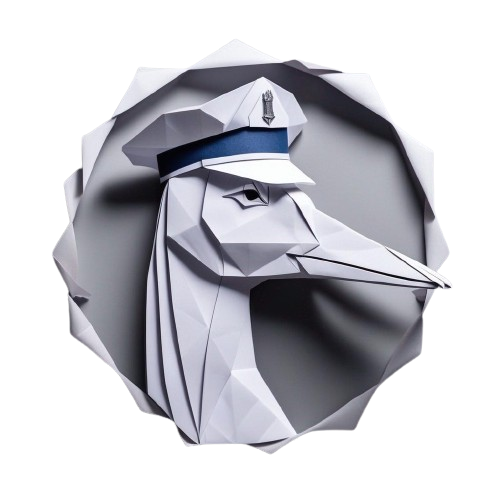
\includegraphics[height=0.8cm]{Gus}};
    \draw[-|,ultra thick,red, decorate, decoration={random steps,segment length=3pt,amplitude=0.5pt}] (A) -- (B) node[midway, left] {4 km};
    \draw[->,ultra thick,blue, decorate, decoration={random steps,segment length=3pt,amplitude=0.5pt}] (B) -- (C) node[midway, left] {3 km};
    \draw[->,ultra thick,violet, decorate, decoration={random steps,segment length=3pt,amplitude=0.5pt}] (C) -- (D) node[midway, left] {1 km};
    
    \node [inner sep=0pt] at (Dp) {
\includegraphics[height=0.8cm]{DuckieGami}};
    \draw[->,ultra thick,red, decorate, decoration={random steps,segment length=3pt,amplitude=0.5pt}] (Ap) -- (Bp) node[midway, left] {4 km};
    \draw[-|,ultra thick,blue, decorate, decoration={random steps,segment length=3pt,amplitude=0.5pt}] (Bp) -- (Cp) node[midway, left] {3 km};
    \draw[->,ultra thick,violet, decorate, decoration={random steps,segment length=3pt,amplitude=0.5pt}] (Cp) -- (Dp) node[midway, left] {1 km};
    
    \draw [decorate, 
	decoration = {brace,mirror,
		raise=15pt,}] (Ap) -- (Dp) node[midway, right, xshift=0.5cm] {27 km};
\end{tikzpicture}}
%Additive Commutativity
\subchapter{Additive Commutativity}
{Duckie and Güs decided that to break the tie, they needed do another competition. \linebreak Because geese are water animals, swimming is a very important skill, so they decided that that should be their next competition. They each have a different strategy. Güs swam \textbf{140} m, dried off, then swam \textbf{160} m. Duckie instead swam \textbf{160} m, dried off, then swam \textbf{140} m. Did they tie?}
{Yes! Duckie and Güs swam the same amount}
{The order of adding does not matter. In other words: A+B = B+A}
{\begin{tikzpicture}
    \coordinate (A) at (0,0);
    \coordinate (B) at (0,4);
    \coordinate (C) at (0,9);
    \coordinate (Ap) at (1.5,0);
    \coordinate (Bp) at (1.5,5);
    \coordinate (Cp) at (1.5,9);
    
    \node [inner sep=0pt] at (C) {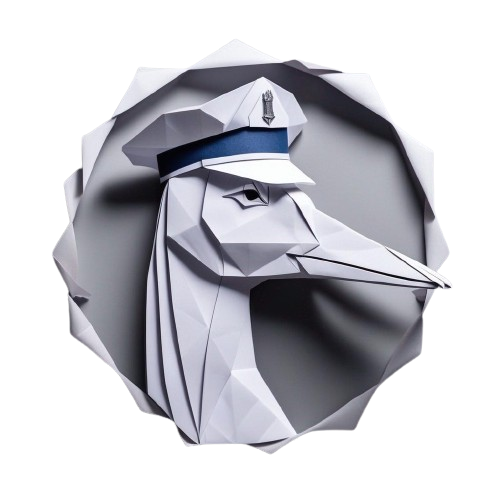
\includegraphics[height=0.8cm]{Gus}};
    \draw[->,ultra thick,red, decorate, decoration={random steps,segment length=3pt,amplitude=0.5pt}] (A) -- (B) node[midway, left] {140 m};
    \draw[->,ultra thick,blue, decorate, decoration={random steps,segment length=3pt,amplitude=0.5pt}] (B) -- (C) node[midway, left] {160 m};
    
    \node [inner sep=0pt] at (Cp) {
\includegraphics[height=0.8cm]{DuckieGami}};
    \draw[->,ultra thick,blue, decorate, decoration={random steps,segment length=3pt,amplitude=0.5pt}] (Ap) -- (Bp) node[midway, left] {160 m};
    \draw[->,ultra thick,red, decorate, decoration={random steps,segment length=3pt,amplitude=0.5pt}] (Bp) -- (Cp) node[midway, left] {140 m};
    
    \draw [decorate, 
	decoration = {brace,mirror,
		raise=15pt,}] (Ap) -- (Cp) node[midway, right, xshift=0.6cm] {300 m};
\end{tikzpicture}}
%Distributativity
\subchapter{Distributivity}
{Duckie and Güs were starting to get frustrated. No matter what happened, the seemed to tie every time! Duckie had thought that if he competed long enough, Güs would get tired and he would be able to win, so challenged him to another flying contest. In the third contest, Güs traveled \textbf{5} km, then \textbf{3} km, and repeated that pattern \textbf{2} times. Duckie instead traveled \textbf{5} km \textbf{2} times, then \textbf{3} km \textbf{2} times. Did they tie?}
{Yes! Duckie and Güs flew the same amount}
{Multiplying by a full expression is the same as multiplying by each part of the expression. In other words: A*(B+C) = (A*B) + (A*C)}
{\begin{tikzpicture}
    \coordinate (A) at (0,0);
    \coordinate (B) at (0,4);
    \coordinate (C) at (0,9);
    \coordinate (Ap) at (1.5,0);
    \coordinate (Bp) at (1.5,5);
    \coordinate (Cp) at (1.5,9);
    
    \node [inner sep=0pt] at (C) {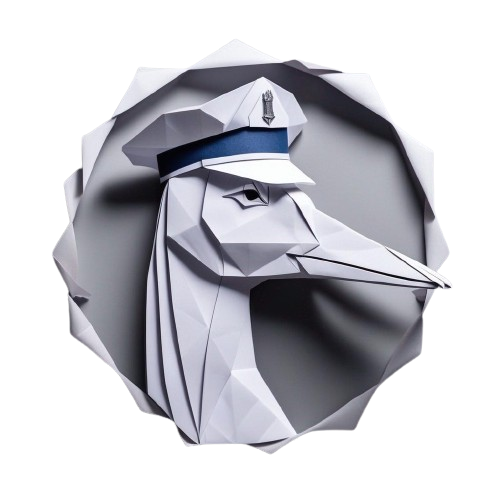
\includegraphics[height=0.8cm]{Gus}};
    \draw[->,ultra thick,red, decorate, decoration={random steps,segment length=3pt,amplitude=0.5pt}] (A) -- (B) node[midway, left] {140 m};
    \draw[->,ultra thick,blue, decorate, decoration={random steps,segment length=3pt,amplitude=0.5pt}] (B) -- (C) node[midway, left] {160 m};
    
    \node [inner sep=0pt] at (Cp) {
\includegraphics[height=0.8cm]{DuckieGami}};
    \draw[->,ultra thick,blue, decorate, decoration={random steps,segment length=3pt,amplitude=0.5pt}] (Ap) -- (Bp) node[midway, left] {160 m};
    \draw[->,ultra thick,red, decorate, decoration={random steps,segment length=3pt,amplitude=0.5pt}] (Bp) -- (Cp) node[midway, left] {140 m};
    
    \draw [decorate, 
	decoration = {brace,mirror,
		raise=15pt,}] (Ap) -- (Cp) node[midway, right, xshift=0.6cm] {300 m};
\end{tikzpicture}}
%Commutativity
\subchapter{Multiplicative Commutativity}
{At this point, Güs realized that Duckie was a very capable goose. When he first challenged Duckie, he expected winning to be a cakewalk, but his opponent ended up posing quite a challenge. Being an honorable goose, this made him respect Duckie more. He decided that the next contest should be a weightlifting competition, where whoever lifted the most amount of total weight would win. Duckie lifted \textbf{10} kg \textbf{3} times, whereas Güs lifted only \textbf{3} kg but does it \textbf{10} times. Did they tie?}
{Yes! Duckie and Güs lifted the same amount}
{The order of multiplication does not affect the result. In other words: A * B = B * A}
{MultiplicativeCommutativity}
%End Of Chapter 2
\paragraph{} After the competition, Duckie and Güs sat down, exhausted. They had both realized that, no matter what competition they had, they were equally matched. Neither one would be able to beat the other, and they had won each other's respect. 
\paragraph{} "Why don't you join me?" asked Duckie.
\paragraph{} "I can't!" Güs cried. "What about my life in the goose police?"
\paragraph{} "Well, do you believe the golden goose is out there?"
\paragraph{} "Honestly, I'm not sure, but if the stories are true, it could change the world"
\paragraph{} Duckie agreed. He knew that there was the possibility the golden goose was a hoax, but believed the positive implications outweighed the dangers of disobeying the goose authorities. 
\paragraph{} "You joined the goose police to help people", he reasoned. "You are clearly strong and capable of making the dangerous journey, and if you can join me, you could do exactly that"
\paragraph{} Güs knew he was right. While he was afraid of what could happen along the journey, he decided to be brave and join Duckie. 
\paragraph{} "All right. I will join you!", he said resolutely. 
\chapter{Essential Algebra}
\paragraph{} Meanwhile, Duckie and Güs's various competitions made the goose authorities a bit confused. Because of Duckie and Güs's "she-goose-igans", they lost track of where Duckie was. They decided that they needed to review their records of Duckie and Güs's locations, and try to figure out what they were doing on the 5th day. 
\vfill
\pagebreak
%Equality
\subchapter{Equality}
{Because Duckie and Güs were travelling together, they were always at the same position at any time.}
{Güs's position = Duckie's position. Duckie's position was P4, so Güs's position was also P4}
{When two things are the same, we write this in mathematics as "="}
{Equality}
%The Equality Rule
\subchapter{The Equality Rule}
{The goose authorities, having trained Güs in the police academy, knew he was a very fast flyer. In fact, he had won the village racing competition for the past three years! Because Duckie and Güs were travelling together, they realized that every time Güs had flown ahead of Duckie, Duckie had to increase his position by the same amount to keep up.}
{Duckie's position + $\Delta$x = Güs's position + $\Delta$x}
{What happens to one side of an equation must happen to the other side so that they are still equal.}
{EqualityRule}
%Commutativity
\subchapter{Variables}
{The goose authorities were still a bit confused about Duckie and Güs's progress. They knew that there were 4 competitions, and that they started at P4. They also knew that they ended at P5. How much did they travel on average in each competition?}
{\begin{center} 4x + 30 = 54 \linebreak 4x + 30 - 30 = 54 - 30 \linebreak $\frac{4x}{4}$ = $\frac{24}{4}$ \linebreak x = $8$  \end{center}}
{Letters and Symbols can be used to represent a number which isn’t already known, such as X. 2x + 3 = 6 means that 2*(some number) + 3 = 6.}
{Variables}
\chapter{Ratios and Fractions}
\paragraph{} It took alot of work, but the authorities finally figured out where Duckie was. They noticed that Duckie and Güs made quite a bit of progress, which was very bad news for them. They wanted to use this information to try to stop them. Because of Güs defecting to join Duckie's journey, they realized that sending other policegeese would make it hard to keep their power in the village. 
\paragraph{} Through their past migrations, they knew lots of bounty hunters along the way, and they believed that they could have them set traps. These bounty hunters were famously clever, and each of them decided to use specific strategies to help them catch Duckie and Güs.
\vfill
\pagebreak
%Ratios
\subchapter{Ratios}
{The first bounty hunter decided to look at the entire journey, and set up traps every P4 km. He estimated that the entire journey was R km long. Duckie having guessed this fairly obvious scheme,  thought that if he knew how many traps there would be, he could avoid them. For every km in the entire journey, there would be a trap every P4 km. How many traps will there be on the journey?}{For every P4 km Duckie has to travel out of (R) km overall, there will be a trap. That means that there is a trap every $\frac{R}{P4}$ km of the journey. For every one km in P4, there are S km in the journey (R), which means that there are S lengths of size P4 within R. There are $\frac{S}{1}$, or S traps}{A ratio is a certain amount for each of another amount, and is written as $\frac{A}{B}$. Break up A into B equal parts}{Blank}
%Multiplying with Fractions
\subchapter{Multiplying with Fractions}
{Using this knowledge, Duckie figured out how to avoid the first bounty hunter's traps. The second bounty hunter decided to prepare better than the first hunter. He realized that km are a very large unit for geese, so decided to start measuring the distance Duckie and Güs flew in a unit he created called "goosemeters" (gm). This meant that he needed to change their position from kilometers into goosemeters. There are U gm for every V m. To help beat the second bounty hunter, Duckie and Güs decide to also measure using gms. How many gms are in P4 km?}{
$\frac{Ugm}{Vm}*\frac{Rm}{1}*\frac{1}{S}=\frac{UR}{VS} gm$
}{Like any number, multiplying by a ratio represents scaling by a certain amount. Imagine a rubber band which is P long, which you can stretch and squish. Multiplication represents scaling the band such that $P*\frac{A}{B}$ is the new length of the band. This is the same as $\frac{P*A}{B}$, or $\frac{P}{B}*A$. This can be seen as dividing the band into B equal parts, then taking one of those parts A times. \paragraph{} Notice that that $\frac{A}{B}$ can create numbers in between 0, 1, 2, etc.}{MultiplyingFractions.png}
%Comparing Fractions
\subchapter{Comparing Fractions}
{Duckie thought that if he traveled enough in one day, the bounty hunter would become confused and leave them alone. On the eighth day, Duckie and Güs traveled an additional W/X of the journey. If Duckie traveled more on the eighth day than the combined previous 7 days, the bounty hunter would become confused and stop chasing Duckie. Has Duckie managed to confuse the bounty hunter?}{Duckie realizes that \begin{center}
    $\frac{X}{X}=1$ \linebreak
    $\frac{UR}{VS}$ * 1 = $\frac{UR}{VS}$ \linebreak
    $\frac{UR}{VS}$ * $\frac{X}{X}$ = $\frac{UR}{VS}$ = $\frac{URX}{VSX}$\linebreak  Which means $\frac{UR}{VS}$  is same as  $\frac{URX}{VSX}$ \linebreak\linebreak
    \textit{similarly}
    $\frac{W}{X}$ =$\frac{WVS}{VSX}$
\end{center}
\paragraph{} Now, we can compare the equal size parts together. $\frac{WVS}{VSX} < \frac{URX}{VSX}$}{We can only deal with fractions together using same-size parts. We can chop up one fraction by multiplying it by another fraction equal to one. If the \textit{denominator}s (the bottom number of the fractions) are the same, the fractions have same sized parts}{ComparingFractions}
%Adding Fractions
\subchapter{Adding Fractions}
{Despite Duckie's best efforts, he was unfortunately not able to confuse the bounty hunter. He was starting to get worried, but Güs had a genius idea. If they could find out where they were along the journey, they might have been able find a new route, which would take them away from the hunter's grasp! They traveled $\frac{WVS}{VSX}$, then they traveled $\frac{URX}{VSX}$. How much of the journey have Duckie and Güs traveled?}{Duckie and Güs have traveled
$\frac{WVS}{VSX}+\frac{URX}{VSX}\linebreak=\frac{WVS+URX}{VSX}\linebreak=\frac{WVS+URX}{VSX}$ths of the journey.}{When adding fractions, break up each fraction so that they are in terms of same-size parts (or having a common denominator). Then, add the numerators as usual.}{AddingFractions}
\paragraph{} Duckie and Güs sighed in relief. After running for bounty hunters for two days and two nights, they were exhausted. They decided to travel slower for a few days and enjoy the scenery. 
\paragraph{} "I can't believe how persistent the goose authorities are." Duckie sighed. "I knew this journey would be tough, but I wasn't expecting bounty hunters!"
\paragraph{} Güs considered this. He had worked with the goose authorities, and knew their patterns. He realized how unusual this was. "I agree, the authorities must really be desparate".
\paragraph{} Just as Duckie opened his beak to reply, he felt a sudden weight on his shoulder's, and began spiraling out of control. It was a net! Another bounty hunter must have set a trap! He started falling down fast, gaining speed as he went. \textbf{Crash!}. Duckie fell to the ground with a thud. Güs hurriedly landed next to him. 
\paragraph{} "Are you alright Duckie‽" he cried in alarm.
\paragraph{} "I'm all right, but I think I need to rest my wing for a few days", Duckie winced. He felt that he hadn't broken a wing, but saw some bruising, and knew he would need time to heal. 
 \paragraph{} "The forest is dangerous though! We can't stay here in the open with all the predators!"
 \paragraph{} "I think my friend Bessie the cow's farm is close enough to walk to from here," Duckie said. "I think she will be able to help keep us safe from the goose authorities."
 \paragraph{} Together, they waddled to Bessie's farm.
 \chapter{Rectangles, Perimeter, and Area}
 \paragraph{} After walking all afternoon, Duckie and Güs finally arrived at Bessie's farm. Despite the bad luck with the net, it was a beautiful afternoon, and the pair couldn't help but feel a sense of calm as the walked up to Bessie's barn.
 \paragraph{} Bessie was sitting outside, chewing on some grass 
 \paragraph{} "Hey there Duckie! Hello Güs! How's it going?" She moo'd
 \paragraph{} "Hi Bessie", Duckie greeted. "I'm looking for the golden goose of legend, and I need some help"
 \paragraph{} "Of course! What do you need?" asked Bessie.
 \paragraph{} "I hurt my wing, and I need to rest here for a few days. The goose authorities sent some bounty hunters after me, and I need you to keep me safe from them", Duckie asked hesitantly.
 \paragraph{} "Wow, that sounds serious. Feel free to stay as long as you like" Bessie turned around to look at Güs. "While Duckie's is getting better, I could use some help on the farm. It's grass-planting season, and it would be much appreciated if you could hlep me out on the farm"
 \paragraph{} Güs, enthusiastically agreed, "That sounds great!"
%Area of Rectangles
 \subchapter{Area of Rectangles}
{On the 9th day of the journey, Güs began working on the farm. His first task was to fly around and scatter grass seeds on the farm. As he went into the store room to find the bags of seeds, he realized he needed to know how many bags of seeds he needs to bring with him. Bessie told him that each bag of seeds can cover a square of grass that is 1 m wide and 1 m across. Güs also knows that the farm is Y m wide and Z m across. How many bags of seeds does Güs need to carry?}{There are Y columns of grass, where each column is made of Z 1x1 squares. This means that there are Y*Z = Y*Z meters squared of grass, and that Güs needs to carry Y*Z bags}{Area is how much space an object takes up. When measuring a 2d shape, we find how many 1x1 squares the object fills. When measuring the area of a 3d shape, we find how many 1x1x1 squares the object fills. Multiplying the length of each side together for "square" shapes gives us the area. (We will discuss area further with integrals)
}{RectangleArea}
%Area of Square Edge Triangles
\subchapter{Area of Square Edge Triangles}{As Güs took off, he noticed that the farm was split into two equal parts along the diagonal to make space for Bessie's pet human Farmer John. He realized that here, he could not plant grass, as Farmer John needed it for corn. How many bags of grass should Güs plant?}{The farm is divided in half, so Güs only needs to plant half of his bags. $\frac{1}{2}*Y*Z =\frac{1}{2}*Y*Z$}{Right triangles (triangles with square edges), are rectangles that have been split in half along the diagonal. This means that the area of a right triangle with side lengths x and y has an area of $\frac{X*Y}{2}$.
}{TriangleArea}
\subchapter{Pythagorean Theorem}{Güs started planting grass. He remembered from school that grass spread rapidly, and so decided that to keep Farmer John's corn safe, he would make a small fence along the diagonal. How long of a fence does Güs need to plant?.}{$Y*Y + Z*Z = Diagonal*Diagonal$}{In a right triangle, the lengths of sides are related to one another. In such a triangle, a*a + b*b = c*c, where c is the diagonal length in the triangle. This relationship is called the \textit{pythagorean theorem} \footnote{A proof of the theorem is found here: \url{https://www.mathsisfun.com/geometry/pythagorean-theorem-proof.html}}}{PythagoreanTheorem}
%Perimeter
\subchapter{Perimeter of a Shape}{After Güs finished planting grass, he decided to take a break for lunch. \paragraph{} "Aaaah", he sighed, contented. As he looked out at the farm, he noticed a discontented look on Bessie's face. \paragraph{}"What's the issue?" he asked. \paragraph{} "It's this fence," Bessie replied. "It's falling apart and we have to look at it all day." Güs decided that to thank her for letting them stay for the night, he would buy her a new fence. How many meters of fence does Güs need to buy?}{Two sides of the fence are Y m long, and two sides of the fence are Z m long. That means that there are Y m + Y m + Z m + Z m = 2*Y m+ 2*Z = 2(Ym+Zm) = 2*Z = 2(Y+Z) m of fence}{ Surface is the size of the edge of an object. When measuring a 2d shape, we find how many 1 long lines fit around the object. When measuring a 3d shape, we find how many 1x1 squares fit around the object. (We will discuss this further with integrals)
The perimeter is the sum of all of the side lengths. Because 2 of the side length of the sides of a rectangle are always the same, 2x+2y is its perimeter, which can also be written as 2(x+y)}{Perimeter}
\section{Shoelace Theorem}
\paragraph{} The shoelace formula is a tool which lets us find the area of any polygon. Go around the vertex's of the polygon, where the current vertex's coordinates are $x_i, y_i$ and the next vertex's coordinates are $x_{i+1}, y_{i+1}$ \linebreak
$A:={\frac{1}{2}}\sum_{cyc} (x_iy_{i+1}-x_{i+1}y_i)$ 
\chapter{Circles and Angles}
\paragraph{} On the 10th day, Bessie had an issue: Farmer John was bored and kept causing trouble on the farm. Rather than letting her and the other cows graze, he was trying to cut down their grass. To keep him entertained and away from the grass, Bessie decided to create crop circles in the corn field.
\paragraph{} "Duckie!", she called. "Want to help make some crop circles?"
\paragraph{} "Sure! I think it will be great for helping my wing recover as well" Duckie replied.
\vfill
\pagebreak
 \subchapter{Angles}
 {Bessie and Duckie came up with a plan to draw their circles. They decided that Duckie would fly around Bessie, staying exactly Q m away from Bessie at each point. To make sure Duckie is exactly the same distance, Bessie would spin around and look at him at any given point. Bessie knows she will get dizzy if she spins too much, so decides to keep track of how much she has turned at any moment.}
 {}
 {The number of meters between the Duckie and Bessie is called r, or the “radius”. When Duckie has flown r meters around Bessie, the amount Güs has turned is a “radian”.}
 {Addition}
 \subchapter{Drawing a single Circle}
 {Bessie and Duckie began to draw the first circle, but ran into an issue. She didn't know when to stop spinning! How many radians does Bessie have to turn so that Duckie makes a full circle (and she looks in the same place she started)?}
 {}
 {When Duckie has flew a full circle around Bessie and Bessie was looking in the same direction where she started, she had turned around 2$\pi$ radians. This amount Bessie turned cannot be written as a fraction, and so is called “irrational”. This specific irrational number has the name “pi”. 
 \paragraph{} For convenience, approximate $\pi$ to be $\frac{22}{7}$ (the actual value of pi is slightly smaller).}
 {Addition}
  \subchapter{Perimeter of a Circle}
 {After some effort calculating, Duckie drew one full circle around Bessie. But, because of his injured wing, he began to feel a bit tired. He decided that in the full day, he would only fly W m so that his wing would recover properly. How much has Duckie flown?}
 {For every radian Bessie turned, Duckie flew R m. Because Bessie turned 2$\pi$ radians, Duckie must have turned $2\pi Q$ m}
 {The perimeter of a circle is always $2\pi r$, where r is radius of the circle}
 {Addition}
 \subchapter{Trigonometric Functions}
 {After resting for a few minutes, Duckie and Bessie started drawing their next circle. They decided that, to help give Farmer John some contrast, they would make it have a radius of 1. While creating the circle, tragedy struck! Duckies lost track of how much he flew. He sees that Bessie turned $\frac{\pi}{4}$ radians. What is Duckie's vertical position? What is Duckie's horizontal position?}
 {}
 {Take a line of length 1. As we rotate the line, we can see it has both a height and a width. When it starts, it has width but not height. When it rotates $\frac{\pi}{2}$ radians it has height but not width. When x is the angle rotated, the width at each angle (or the adjacent side/the diagonal side) is cos(x). The height at each angle (or the opposite side/the diagonal side) is sin(x). If the line is}
 {Addition}
  \subchapter{Trigonometric Identities}
 {Duckie, tired, but with a healed wing, sat down. He and Bessie were ready to take the day off, and he was ready to start flying the next day. Güs, who had been planting grass, walked over to them. 
 \paragraph{} "Hey Guys! How was your work in the cornfield?"
 \paragraph{} "It was pretty good!" Bessie replied. "We were drawing circles for Farmer John while you planted grass"
 \paragraph{} Güs looked at Bessie in surprise. "That's what you were doing? I thought you were tracing the point of an arrow where the width\texttimes the width plus the height \texttimes the height equaled one!"
 The trio looked at each other in confusion. Who is right?}
 {They were all right! The width of the arrow is cos(x), and the height of the arrow is sin(x). Through pythagorean theorem, the length of the arrow must be 1, which is also the radius that Duckie flew.}
 {sin(x) * sin(x) + cos(x) * cos(x) = 1*1 = 1}
 {Addition}
\end{document}